\documentclass[12pt,a4paper]{article}

\usepackage[utf8]{inputenc}
\usepackage[T1]{fontenc}
\usepackage[italian]{babel}
\usepackage{geometry}
\usepackage{graphicx}
\usepackage{booktabs}
\usepackage{float}
\usepackage{amsmath}
\usepackage{caption}
\usepackage{array}
\usepackage{tabularx}
\usepackage{hyperref}

\geometry{
    top=2.5cm,
    bottom=2.5cm,
    left=3.5cm,
    right=3.5cm
}

% Paragrafi allineati allo stesso margine sinistro
\setlength{\parindent}{0pt}
\setlength{\parskip}{0.65em}

% Didascalia sopra le tabelle e sotto le figure
\captionsetup[table]{position=top}
\captionsetup[figure]{position=bottom}

\title{Ipossia tumorale e sopravvivenza nell'adenocarcinoma polmonare}
\author{Salvatore Megna}
\date{}

\begin{document}

\maketitle

\section{Introduzione}

L'adenocarcinoma polmonare è una delle principali forme di carcinoma polmonare non a piccole cellule ed è caratterizzato da una marcata eterogeneità clinica e biologica tra i pazienti. Tale eterogeneità può tradursi in differenze rilevanti nella progressione della malattia, nella risposta ai trattamenti e nella sopravvivenza. Per studiare questi aspetti è stato costruito un dataset a partire dai dati clinici e molecolari del progetto TCGA-LUAD PanCancer Atlas (\textit{The Cancer Genome Atlas -- Lung Adenocarcinoma}), integrando per ciascun paziente il tempo di sopravvivenza globale, lo stato vitale, l'età alla diagnosi, il sesso, lo stadio patologico, il sottotipo istologico e alcuni indicatori molecolari associati all'ipossia tumorale.

L'obiettivo specifico dell'analisi è valutare se, e in quale misura, le caratteristiche cliniche e molecolari dei pazienti siano associate alla sopravvivenza globale. In particolare, si vuole comprendere se gli indicatori biologici legati all'ipossia tumorale forniscano informazioni prognostiche aggiuntive rispetto alle principali caratteristiche cliniche, permettendo di individuare profili associati a esiti di sopravvivenza differenti. A tal fine, il tempo di sopravvivenza viene analizzato mediante le curve di Kaplan--Meier, il test di log-rank e il modello semiparametrico di Cox. Vengono inoltre verificate le principali assunzioni del modello mediante opportuni strumenti diagnostici.

\section{Il dataset}

\subsection{Costruzione del dataset}

I dati utilizzati provengono dallo studio TCGA-LUAD PanCancer Atlas e sono stati acquisiti attraverso il portale cBioPortal. Il dataset clinico originario comprende 566 pazienti con adenocarcinoma polmonare e 40 variabili. La struttura dei dati è di tipo patient-level: ciascuna riga corrisponde a un singolo paziente e non sono presenti identificativi duplicati.

Nel presente studio i dati di sopravvivenza sono di tipo \textit{right-censored}. Per i pazienti deceduti è noto il tempo trascorso fino al decesso, mentre per quelli ancora in vita il tempo osservato termina in corrispondenza dell'ultimo contatto disponibile. Le analisi mediante curve di Kaplan--Meier, test di log-rank e modello di Cox assumono che la censura sia indipendente e non informativa rispetto al rischio di morte.

In seguito alla verifica dell'outcome, alla rimozione dei tempi di sopravvivenza nulli e all'esclusione delle osservazioni con dati mancanti nelle covariate utilizzate, il dataset comune ai modelli comprende 485 pazienti, di cui 177 deceduti e 308 censurati. Per ciascun paziente sono state considerate le seguenti informazioni:

\begin{itemize}

    \item \textbf{Tempo di sopravvivenza globale:} numero di mesi trascorsi dalla diagnosi fino alla data del decesso, oppure, in assenza dell'evento, fino alla data dell'ultimo contatto disponibile. Al tempo è associato un indicatore binario che assume valore 1 in caso di decesso e valore 0 in caso di censura.

    \item \textbf{Età alla diagnosi:} età del paziente al momento della diagnosi, espressa in anni. Nei modelli di Cox è stata riscalata in unità di dieci anni, in modo da rendere più immediata l'interpretazione dell'hazard ratio.

    \item \textbf{Sesso:} variabile categoriale distinta nelle modalità Female e Male.

    \item \textbf{Stadio patologico:} classificazione dell'estensione anatomica della malattia secondo il sistema dell'American Joint Committee on Cancer (AJCC). Le categorie originarie IA e IB sono state raggruppate nello stadio I, IIA e IIB nello stadio II, IIIA e IIIB nello stadio III, mentre lo stadio IV è stato mantenuto separato.

    \item \textbf{Sottotipo istologico:} variabile ricavata dal codice istologico ICD-O-3 e suddivisa nelle categorie Adenocarcinoma NOS, Mixed adenocarcinoma e Other subtype.

    \item \textbf{Indicatori molecolari di ipossia tumorale:} score compositi ricavati dall'espressione di insiemi predefiniti di geni coinvolti nella risposta cellulare alla ridotta disponibilità di ossigeno. Non misurano direttamente la concentrazione di ossigeno nel tumore, ma sintetizzano quanto il profilo di espressione genica del campione sia compatibile con un fenotipo ipossico. Valori più elevati indicano, in termini relativi, una maggiore attivazione della firma molecolare di ipossia. Nel dataset erano disponibili Buffa Hypoxia Score, Ragnum Hypoxia Score e Winter Hypoxia Score, già calcolati secondo tre differenti firme geniche.

\end{itemize}

La struttura delle principali variabili considerate è riassunta nella Tabella~\ref{tab:variabili_dataset}.

\begin{table}[H]
\centering
\caption{Principali variabili considerate nell'analisi.}
\label{tab:variabili_dataset}

\renewcommand{\arraystretch}{1.25}
\setlength{\tabcolsep}{8pt}

\begin{tabularx}{\textwidth}{
    >{\raggedright\arraybackslash}p{3.3cm}
    >{\raggedright\arraybackslash}p{2.4cm}
    >{\raggedright\arraybackslash}X
}
\toprule
\textbf{Variabile} & \textbf{Tipo} & \textbf{Descrizione} \\
\midrule

Tempo di sopravvivenza
& Continua
& Tempo di sopravvivenza globale o di follow-up, espresso in mesi. \\

Evento
& Binaria
& Indicatore di evento: 1 in caso di decesso e 0 in caso di censura. \\

Età
& Continua
& Età del paziente al momento della diagnosi, espressa in anni. \\

Sesso
& Categoriale
& Sesso del paziente, distinto nelle modalità Female e Male. \\

Stadio patologico
& Categoriale
& Estensione della malattia raggruppata nelle categorie I, II, III e IV. \\

Sottotipo istologico
& Categoriale
& Sottotipo raggruppato in Adenocarcinoma NOS, Mixed adenocarcinoma e Other subtype. \\

Score di ipossia
& Continua
& Indici compositi di espressione genica associati a un fenotipo tumorale ipossico. \\

\bottomrule
\end{tabularx}
\end{table}

La Tabella~\ref{tab:flusso_pazienti} riassume il passaggio dal dataset originario al campione utilizzato nei modelli multivariati.

\begin{table}[H]
\centering
\caption{Costruzione del campione analitico.}
\label{tab:flusso_pazienti}

\renewcommand{\arraystretch}{1.2}

\begin{tabular}{l r}
\toprule
\textbf{Fase} & \textbf{Numero di pazienti} \\
\midrule
Dataset clinico originario & 566 \\
Outcome di sopravvivenza completo & 505 \\
Outcome valido e tempo maggiore di zero & 501 \\
Dataset comune ai modelli di Cox & 485 \\
\bottomrule
\end{tabular}
\end{table}

\subsection{Dati mancanti}

La presenza di valori mancanti è stata valutata separatamente per l'outcome di sopravvivenza e per le covariate considerate nell'analisi. Nel dataset originario di 566 pazienti, 61 soggetti non disponevano di informazioni complete sul tempo o sullo stato di sopravvivenza e non potevano quindi essere inclusi nelle analisi. Tra i 505 pazienti con outcome completo, quattro presentavano un tempo di osservazione pari a zero e sono stati esclusi, ottenendo un campione di 501 soggetti con outcome valido.

La Tabella~\ref{tab:dati_mancanti} riporta i valori mancanti osservati nelle principali covariate all'interno di questo campione.

\begin{table}[H]
\centering
\caption{Valori mancanti nelle principali covariate del dataset di sopravvivenza.}
\label{tab:dati_mancanti}

\renewcommand{\arraystretch}{1.2}
\setlength{\tabcolsep}{10pt}

\begin{tabular}{l r r}
\toprule
\textbf{Variabile} &
\textbf{Valori mancanti} &
\textbf{Percentuale} \\
\midrule

Età alla diagnosi
& 10
& 2,0\% \\

Sesso
& 0
& 0,0\% \\

Stadio patologico
& 2
& 0,4\% \\

Sottotipo istologico
& 0
& 0,0\% \\

Buffa Hypoxia Score
& 4
& 0,8\% \\

Ragnum Hypoxia Score
& 4
& 0,8\% \\

Winter Hypoxia Score
& 4
& 0,8\% \\

\bottomrule
\end{tabular}
\end{table}

Poiché la quota di dati mancanti nelle covariate risultava complessivamente contenuta, non è stata effettuata alcuna procedura di imputazione. Per garantire che i modelli multivariati fossero stimati sullo stesso insieme di pazienti e che i confronti tra modelli fossero direttamente interpretabili, è stata adottata un'analisi per casi completi.

Sono stati quindi mantenuti soltanto i soggetti con informazioni disponibili per il tempo di sopravvivenza, lo stato dell'evento, l'età, il sesso, lo stadio patologico, il sottotipo istologico e il punteggio di ipossia selezionato per il modello. Il dataset comune alle analisi di Cox comprende pertanto 485 pazienti, corrispondenti al 96,8\% dei 501 soggetti con outcome valido.

La perdita di informazione dovuta all'esclusione dei casi incompleti è quindi limitata. Tuttavia, l'analisi per casi completi presuppone che l'assenza dei dati non introduca differenze sistematiche rilevanti tra i pazienti inclusi e quelli esclusi; tale aspetto rappresenta un limite da considerare nell'interpretazione dei risultati.

% ================================================================
% 3. ANALISI ESPLORATIVA
% ================================================================

% Percorso della cartella caricata su Overleaf
\graphicspath{{grafici_report/}}

\section{Analisi esplorativa}

\subsection{Le variabili}

L'analisi esplorativa è stata condotta sul dataset comune ai modelli di Cox, costituito da 485 pazienti. Sono state esaminate la distribuzione del tempo osservato, l'età alla diagnosi, le principali variabili categoriali e gli indicatori molecolari di ipossia tumorale.

\subsubsection{Tempo di sopravvivenza}

La Figura~\ref{fig:distribuzione_tempo} mostra la distribuzione del tempo di sopravvivenza globale o di follow-up, espresso in mesi.

\begin{figure}[H]
    \centering
    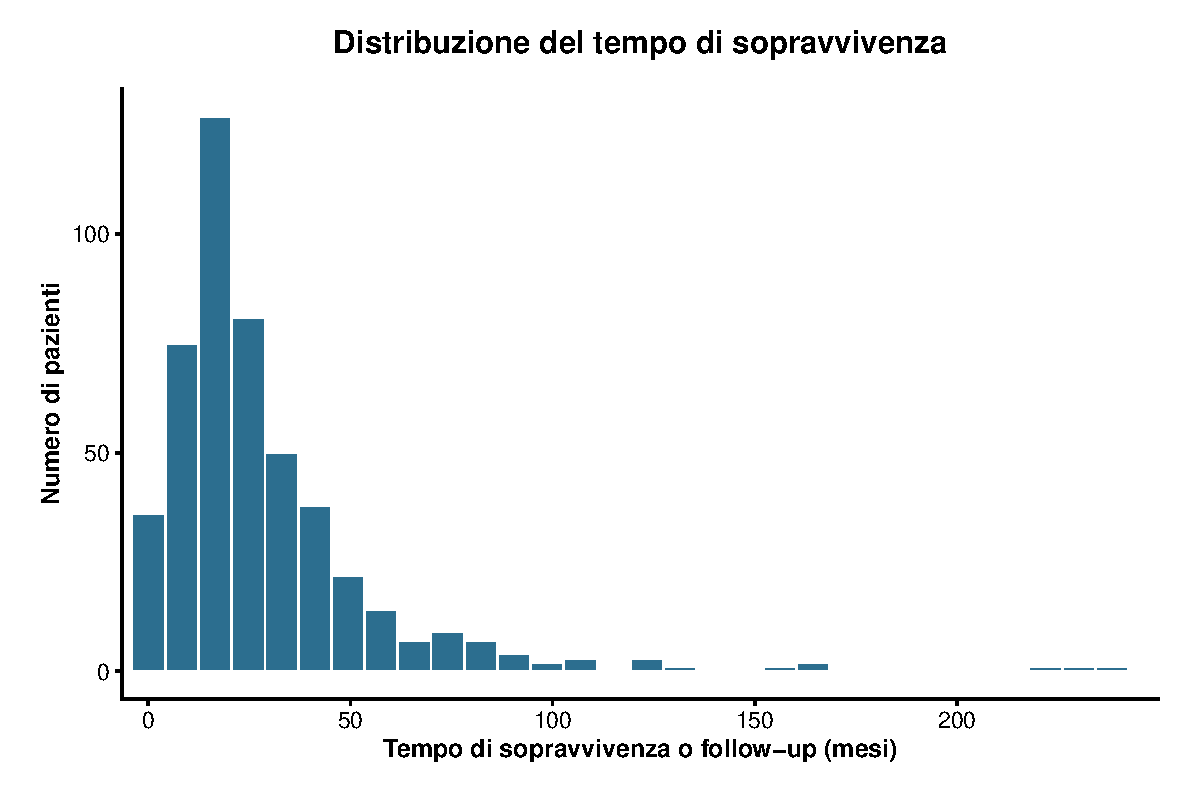
\includegraphics[width=0.92\textwidth]{distribuzione_tempo_sopravvivenza.pdf}
    \caption{Distribuzione del tempo di sopravvivenza o di follow-up.}
    \label{fig:distribuzione_tempo}
\end{figure}

Il tempo osservato presenta una mediana di 21,4 mesi e un intervallo interquartile compreso tra 13,7 e 36,1 mesi; la media è pari a 29,1 mesi. La distribuzione è fortemente asimmetrica verso destra: la maggior parte dei pazienti presenta tempi relativamente contenuti, mentre un numero ridotto di soggetti è seguito per periodi molto più lunghi, fino a 238,3 mesi.

\subsubsection{Età alla diagnosi}

La distribuzione dell'età dei pazienti al momento della diagnosi è riportata nella Figura~\ref{fig:distribuzione_eta}.

\begin{figure}[H]
    \centering
    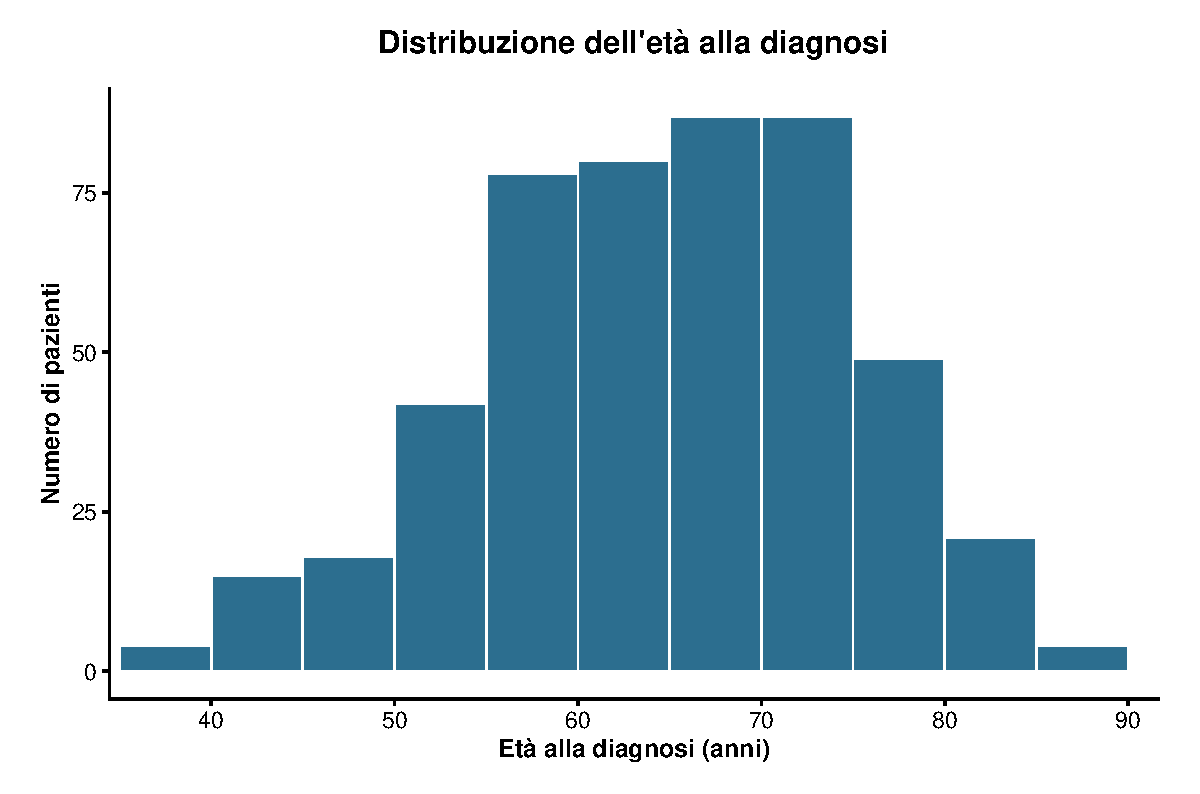
\includegraphics[width=0.92\textwidth]{distribuzione_eta.pdf}
    \caption{Distribuzione dell'età alla diagnosi.}
    \label{fig:distribuzione_eta}
\end{figure}

L'età è concentrata prevalentemente tra circa 55 e 80 anni, con pochi pazienti molto giovani o particolarmente anziani. La distribuzione non mostra anomalie tali da impedire l'impiego dell'età come covariata quantitativa nel modello di Cox.

\subsubsection{Variabili categoriali}

Le distribuzioni del sesso, dello stadio patologico e del sottotipo istologico sono rappresentate separatamente nelle Figure~\ref{fig:distribuzione_sesso}, \ref{fig:distribuzione_stadio} e \ref{fig:distribuzione_istologia}.

\begin{figure}[H]
    \centering
    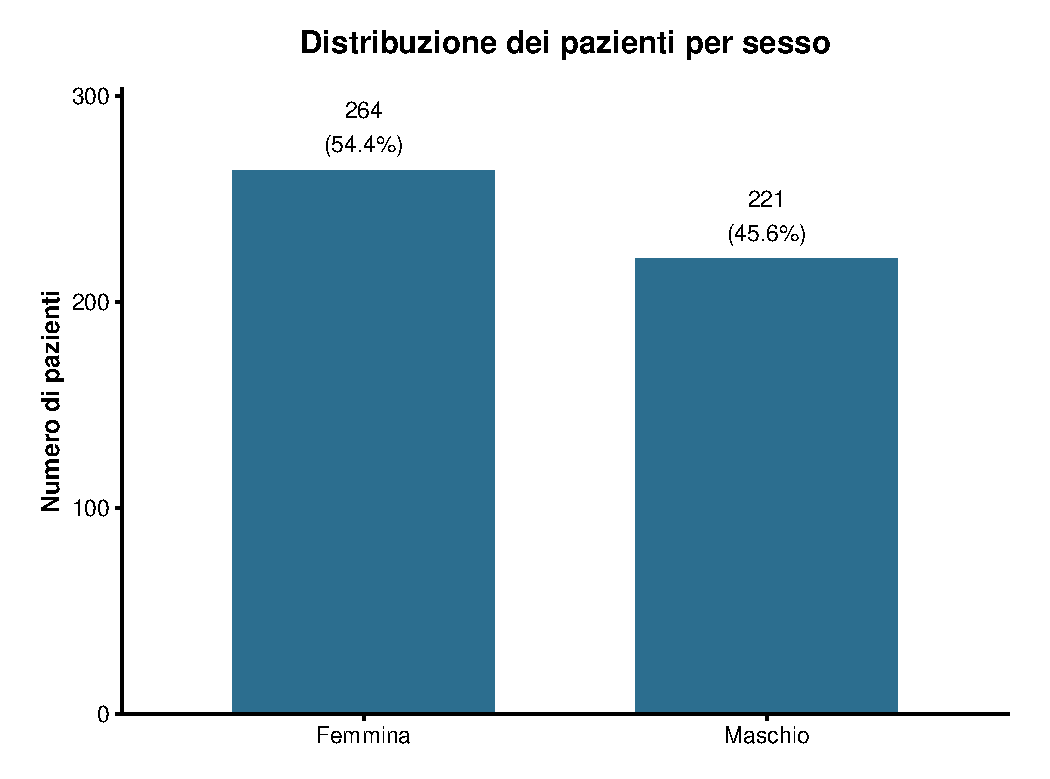
\includegraphics[width=0.78\textwidth]{distribuzione_sesso.pdf}
    \caption{Distribuzione dei pazienti per sesso.}
    \label{fig:distribuzione_sesso}
\end{figure}

Nel campione sono presenti 264 donne, pari al 54,4\% del totale, e 221 uomini, pari al 45,6\%.

\begin{figure}[H]
    \centering
    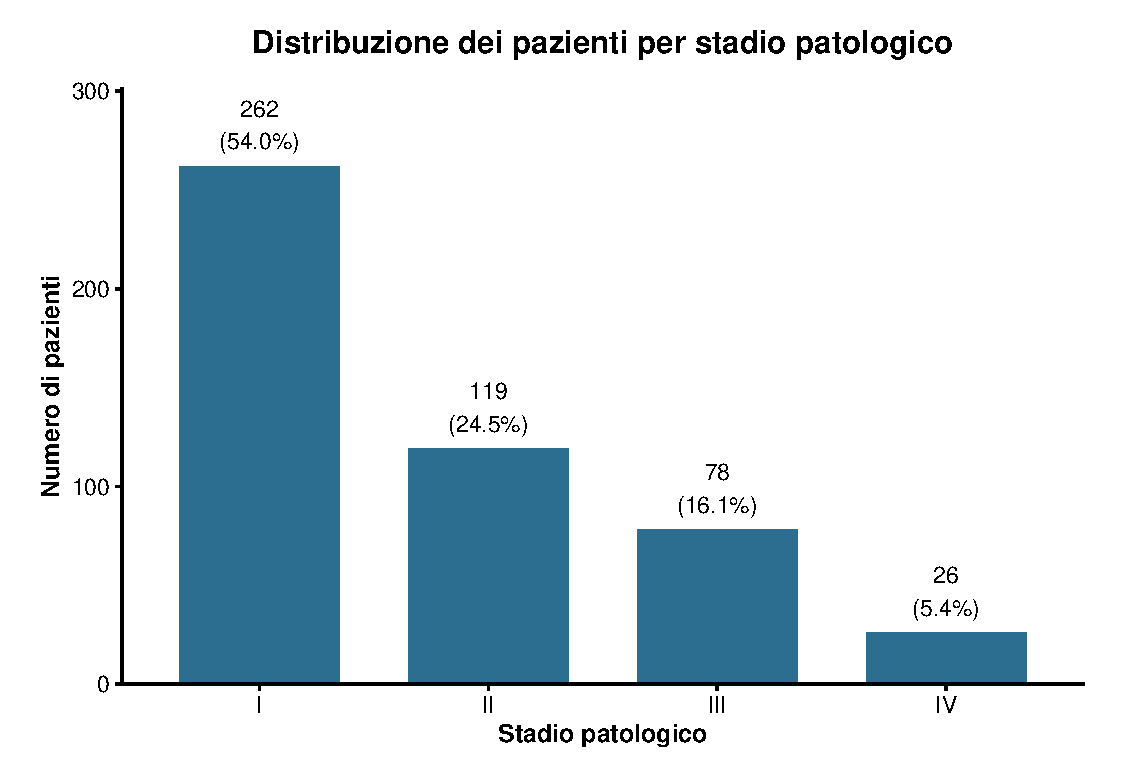
\includegraphics[width=0.82\textwidth]{distribuzione_stadio.pdf}
    \caption{Distribuzione dei pazienti per stadio patologico.}
    \label{fig:distribuzione_stadio}
\end{figure}

La distribuzione è sbilanciata verso gli stadi iniziali: oltre la metà dei pazienti appartiene allo stadio I, mentre lo stadio IV rappresenta soltanto il 5,4\% del campione. Le stime relative allo stadio IV devono quindi essere interpretate con maggiore cautela.

\begin{figure}[H]
    \centering
    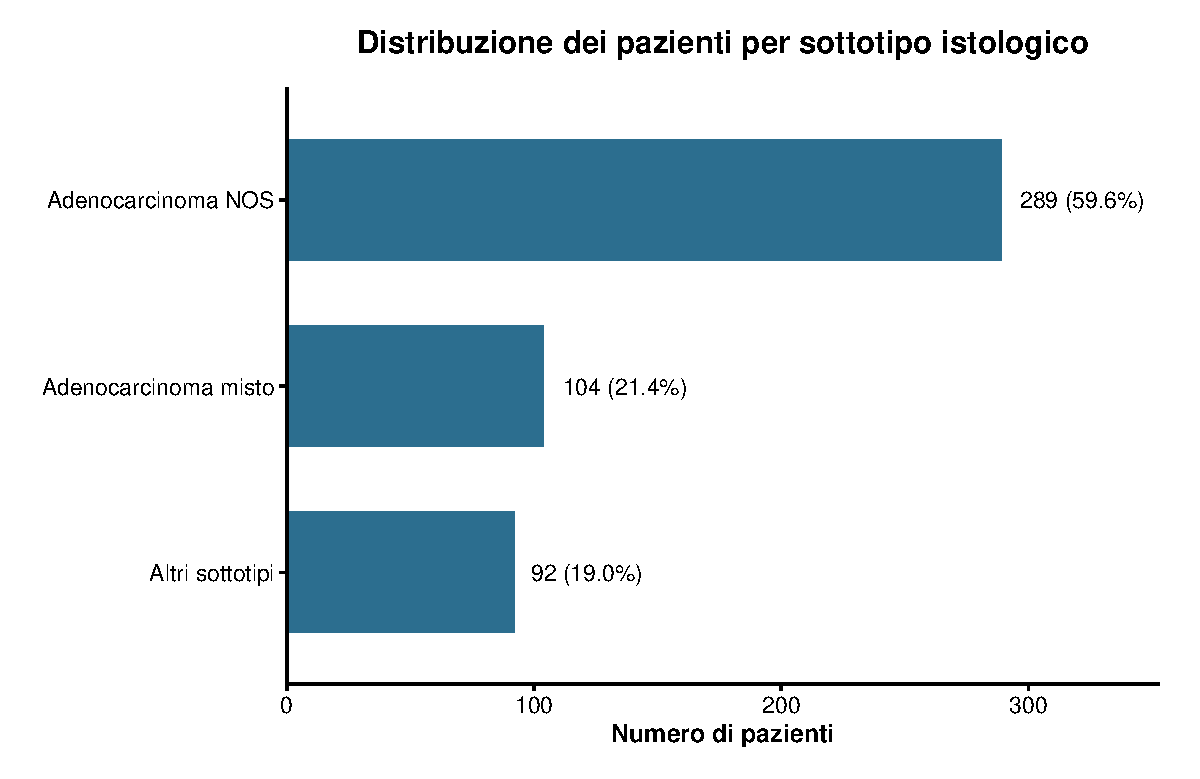
\includegraphics[width=0.88\textwidth]{distribuzione_istologia.pdf}
    \caption{Distribuzione dei pazienti per sottotipo istologico.}
    \label{fig:distribuzione_istologia}
\end{figure}

L'Adenocarcinoma NOS costituisce la categoria prevalente, comprendendo circa il 60\% del campione. La categoria Altri sottotipi è meno numerosa e riunisce forme istologiche differenti, risultando quindi internamente eterogenea.

\subsubsection{Indicatori di ipossia tumorale}

Nel dataset sono disponibili tre score associati all'ipossia tumorale: Buffa Hypoxia Score, Ragnum Hypoxia Score e Winter Hypoxia Score. Ciascuno sintetizza l'espressione di una diversa firma di geni che rispondono alla carenza di ossigeno. Questi valori non rappresentano quindi una misura diretta dell'ossigenazione del tessuto, ma indici molecolari relativi: uno score più elevato indica che il profilo di espressione del tumore è maggiormente compatibile con una risposta ipossica. Poiché le tre firme utilizzano insiemi di geni e scale differenti, i valori assoluti dei tre score non devono essere confrontati direttamente tra loro. Le rispettive distribuzioni sono riportate nella Figura~\ref{fig:distribuzione_hypoxia}.

\begin{figure}[H]
    \centering
    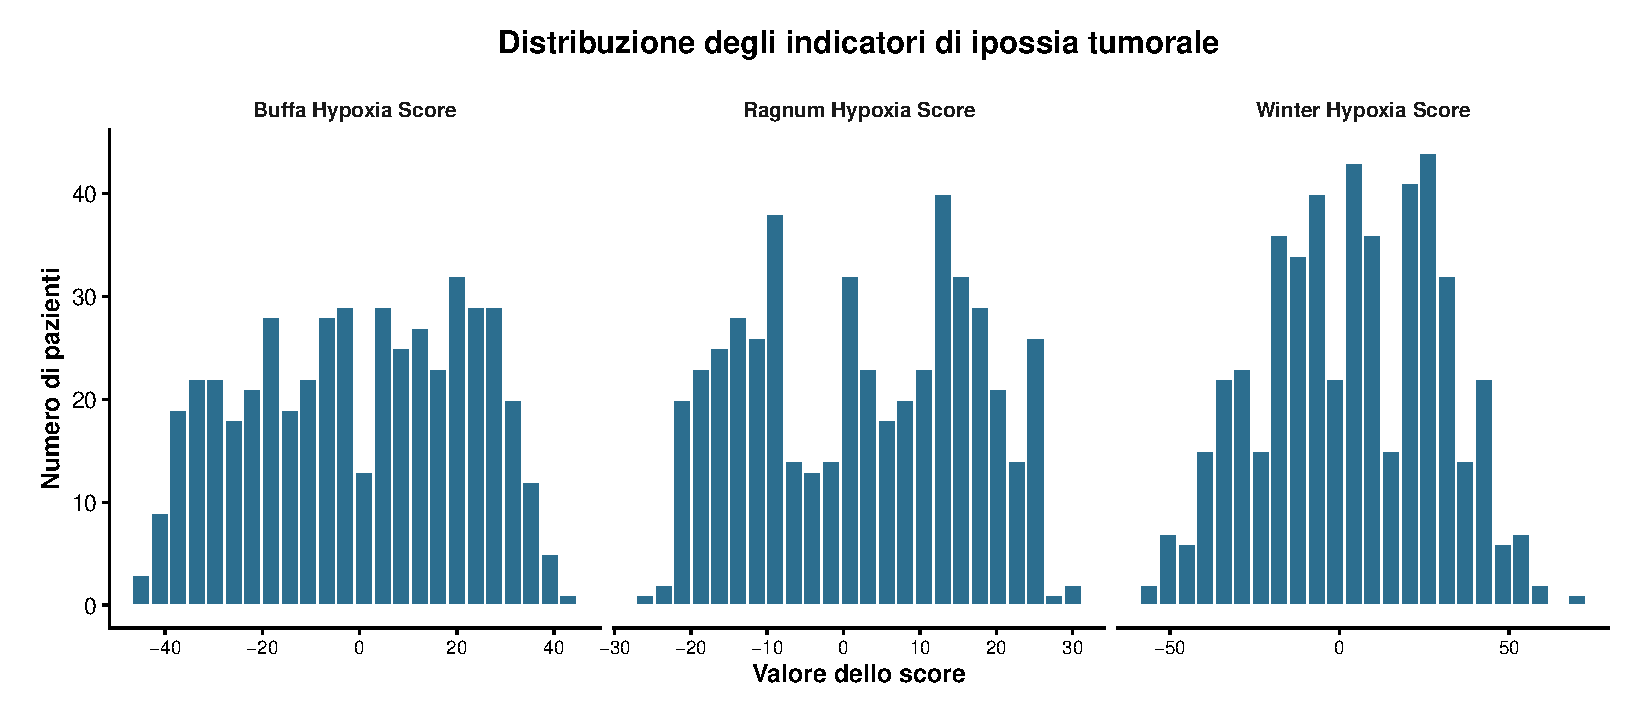
\includegraphics[width=\textwidth]{distribuzione_hypoxia_scores.pdf}
    \caption{Distribuzione degli indicatori molecolari di ipossia tumorale.}
    \label{fig:distribuzione_hypoxia}
\end{figure}

I tre punteggi assumono valori sia negativi sia positivi e presentano distribuzioni abbastanza regolari, senza code estreme tali da richiedere trasformazioni preliminari. Nei modelli sono pertanto considerati inizialmente come variabili quantitative continue. Pur essendo espressi su scale differenti, i tre score possono essere confrontati in termini di associazione lineare mediante il coefficiente di correlazione di Pearson.

\subsection{Correlazioni}

La relazione lineare fra i tre indicatori di ipossia è stata valutata mediante il coefficiente di correlazione di Pearson. La matrice è mostrata nella Figura~\ref{fig:correlazione_hypoxia}.

\begin{figure}[H]
    \centering
    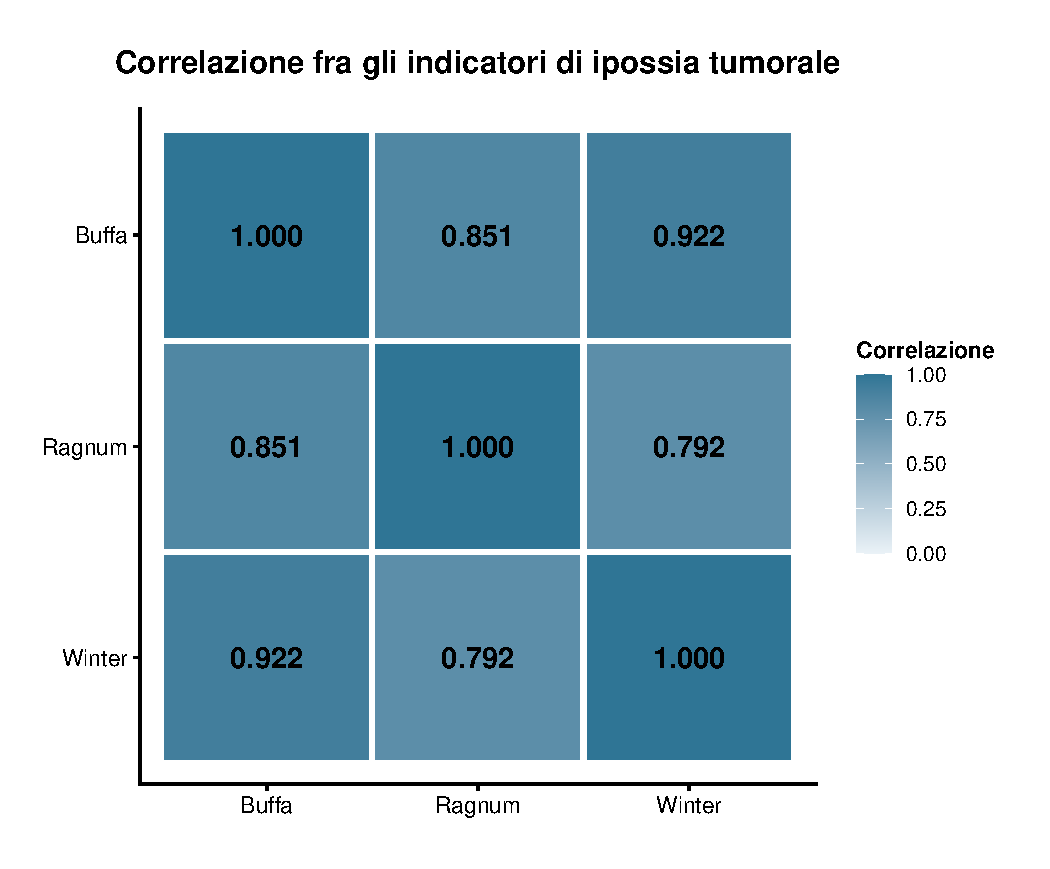
\includegraphics[width=0.76\textwidth]{correlazione_hypoxia_scores.pdf}
    \caption{Matrice di correlazione fra gli indicatori di ipossia tumorale.}
    \label{fig:correlazione_hypoxia}
\end{figure}

Le correlazioni risultano elevate: la correlazione tra Buffa e Ragnum è pari a 0,851, quella tra Buffa e Winter è pari a 0,922, mentre quella tra Ragnum e Winter è pari a 0,792.

\begin{table}[H]
    \centering
    \caption{Correlazioni fra gli indicatori di ipossia tumorale.}
    \label{tab:correlazioni_hypoxia}
    \renewcommand{\arraystretch}{1.2}
    \begin{tabular}{l l c}
        \toprule
        \textbf{Indicatore 1} & \textbf{Indicatore 2} & \textbf{Correlazione} \\
        \midrule
        Buffa  & Ragnum & 0,851 \\
        Buffa  & Winter & 0,922 \\
        Ragnum & Winter & 0,792 \\
        \bottomrule
    \end{tabular}
\end{table}

La forte associazione tra i tre score suggerisce che essi descrivano componenti largamente sovrapposte dello stesso fenomeno biologico. Il loro inserimento simultaneo nel modello potrebbe quindi generare collinearità e rendere instabili le stime. Per mantenere il modello parsimonioso e interpretabile è stato scelto un solo indicatore, individuando nel Buffa Hypoxia Score la firma principale dell'analisi. Ragnum e Winter sono stati utilizzati per verificare la coerenza del fenomeno molecolare, ma non sono stati inseriti contemporaneamente nel modello. La scelta è quindi operativa e non rappresenta una dimostrazione di superiorità formale del Buffa score rispetto agli altri due indicatori.

% ================================================================
% 4. ANALISI DI SOPRAVVIVENZA
% ================================================================

\section{Analisi di sopravvivenza}

La funzione di sopravvivenza è stata stimata mediante il metodo di Kaplan--Meier, considerando come tempo l'intervallo, espresso in mesi, tra la diagnosi e il decesso, oppure, per i pazienti che non hanno presentato l'evento, tra la diagnosi e l'ultimo contatto disponibile. Le osservazioni relative ai pazienti ancora in vita al termine del follow-up sono quindi considerate censurate.

\subsection{Curva di Kaplan--Meier complessiva}

La curva complessiva descrive l'andamento della probabilità di sopravvivenza nella popolazione in studio. Come mostrato nella Figura~\ref{fig:km_complessiva}, la probabilità di sopravvivenza diminuisce progressivamente durante il follow-up, con una riduzione più marcata nei primi anni e una successiva coda caratterizzata da un numero più limitato di pazienti ancora a rischio.

\begin{figure}[H]
    \centering
    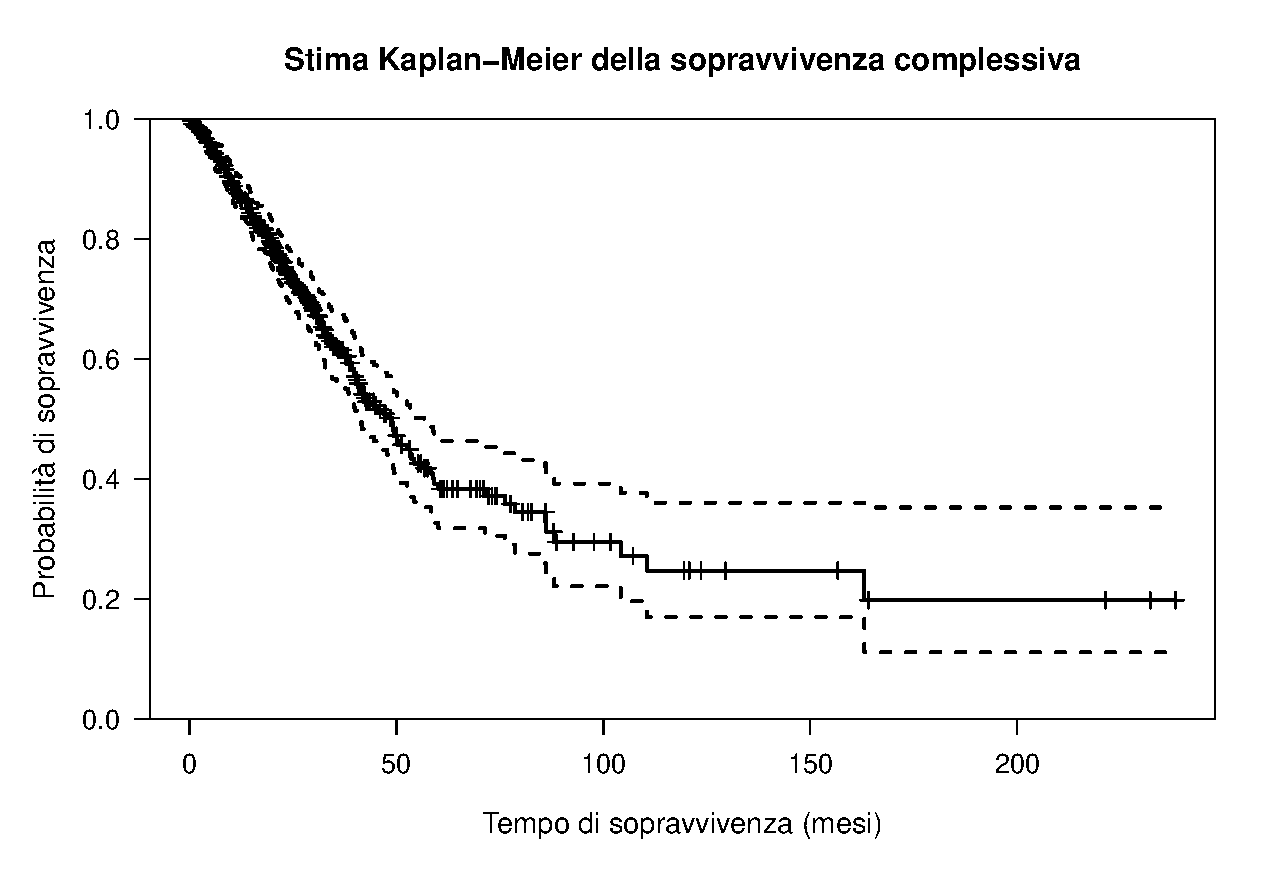
\includegraphics[width=0.92\textwidth]{km_complessiva.pdf}
    \caption{Curva di Kaplan--Meier complessiva con intervallo di confidenza al 95\%.}
    \label{fig:km_complessiva}
\end{figure}

La sopravvivenza mediana stimata è pari a 49,1 mesi, con intervallo di confidenza al 95\% compreso tra 41,4 e 56,7 mesi. La probabilità di sopravvivenza stimata è pari all'87,5\% a 12 mesi, al 61,5\% a 36 mesi e al 39,2\% a 60 mesi.

\subsection{Curve di Kaplan--Meier per stadio patologico}

Per valutare l'associazione tra estensione della malattia e sopravvivenza, sono state stimate curve separate per i quattro stadi patologici, riportate nella Figura~\ref{fig:km_stadio}.

\begin{figure}[H]
    \centering
    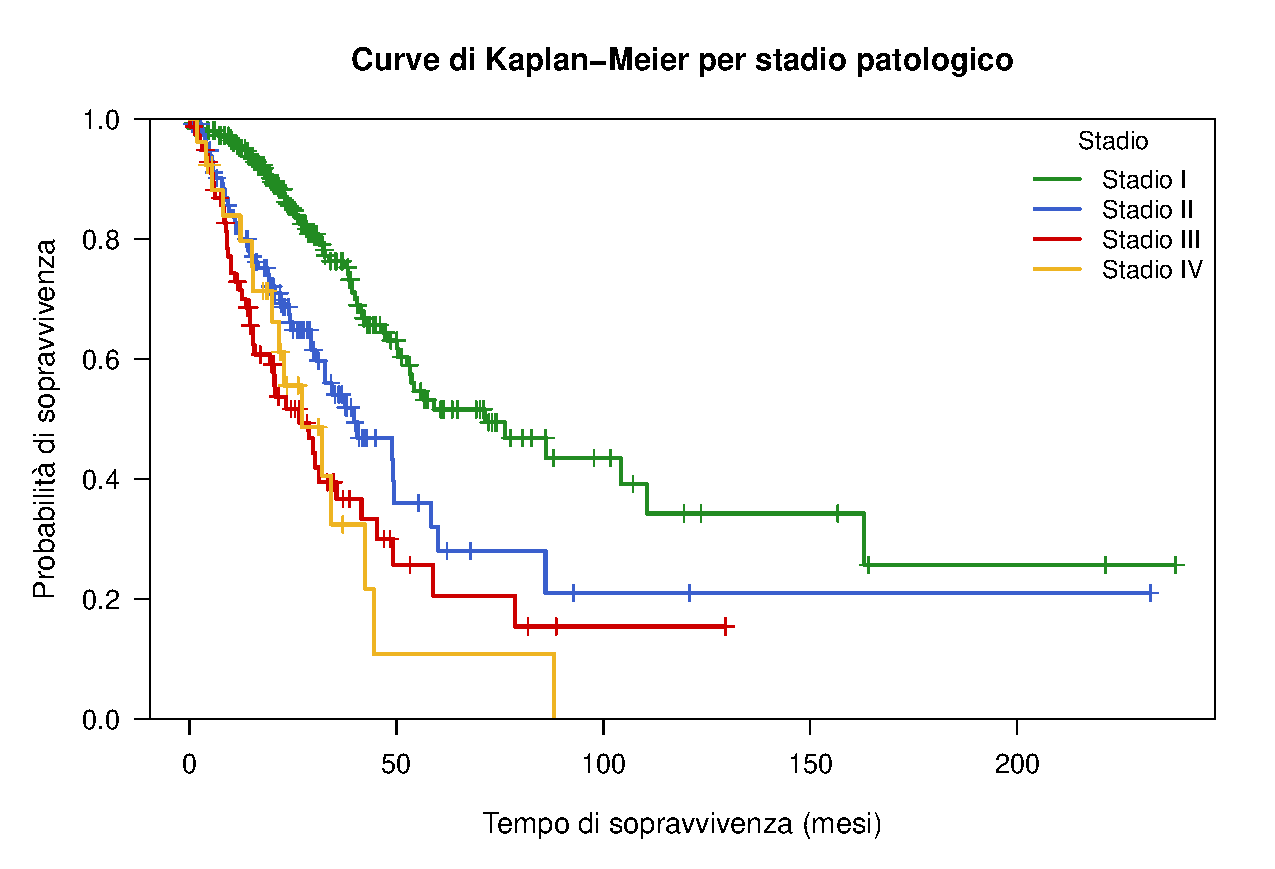
\includegraphics[width=0.92\textwidth]{km_stadio.pdf}
    \caption{Curve di Kaplan--Meier per stadio patologico.}
    \label{fig:km_stadio}
\end{figure}

La curva relativa allo stadio I si mantiene generalmente al di sopra delle altre, indicando una prognosi più favorevole. Gli stadi II, III e IV mostrano invece una progressiva riduzione della probabilità di sopravvivenza, con esiti complessivamente peggiori negli stadi più avanzati.

Il test di log-rank evidenzia una differenza statisticamente significativa tra le curve di sopravvivenza dei quattro gruppi:

\[
p < 0{,}001.
\]

Lo stadio patologico risulta quindi fortemente associato alla sopravvivenza globale nell'analisi non aggiustata. Tale confronto non tiene tuttavia conto delle altre caratteristiche cliniche e molecolari dei pazienti, che verranno considerate successivamente mediante il modello di Cox.

% ================================================================
% 4.2 MODELLO DI COX MULTIVARIATO E STRATIFICATO
% ================================================================

\subsection{Modello di Cox multivariato e stratificato}

Per valutare simultaneamente l'associazione tra le caratteristiche cliniche e molecolari dei pazienti e il rischio di morte è stato inizialmente stimato un modello di Cox multivariato a rischi proporzionali. Il modello comprende l'età alla diagnosi, il sesso, lo stadio patologico, il sottotipo istologico e il Buffa Hypoxia Score.

L'età è stata espressa in unità di dieci anni e il Buffa Hypoxia Score in unità di dieci punti, così da rendere più immediata l'interpretazione dei rispettivi hazard ratio. Le categorie di riferimento sono il sesso femminile, lo stadio I e l'adenocarcinoma NOS.

Il modello iniziale può essere espresso come:

\begin{equation}
\begin{split}
h(t \mid X)=h_0(t)\exp\{&
\beta_1 \mathrm{Et\grave{a}}_{10}
+\beta_2 \mathrm{Sesso}
+\beta_3 \mathrm{Stadio} \\
&+\beta_4 \mathrm{Istologia}
+\beta_5 \mathrm{Buffa}_{10}\}.
\end{split}
\label{eq:cox_standard}
\end{equation}

I risultati del modello multivariato standard sono riportati nella Tabella~\ref{tab:cox_standard}.

\begin{table}[H]
\centering
\caption{Modello di Cox multivariato standard.}
\label{tab:cox_standard}
\renewcommand{\arraystretch}{1.15}
\small
\begin{tabular}{l c c c}
\toprule
\textbf{Covariata}
& \textbf{HR}
& \textbf{IC 95\%}
& \textbf{$p$-value} \\
\midrule
Età, per 10 anni
& 1,236
& 1,052--1,452
& 0,010 \\

Maschio vs Femmina
& 1,013
& 0,750--1,367
& 0,933 \\

Stadio II vs I
& 1,931
& 1,334--2,795
& $<0,001$ \\

Stadio III vs I
& 2,888
& 1,960--4,255
& $<0,001$ \\

Stadio IV vs I
& 3,821
& 2,170--6,729
& $<0,001$ \\

Adenocarcinoma misto vs NOS
& 0,748
& 0,504--1,111
& 0,150 \\

Altri sottotipi vs NOS
& 0,477
& 0,282--0,807
& 0,006 \\

Buffa score, per 10 punti
& 1,117
& 1,036--1,206
& 0,004 \\
\bottomrule
\end{tabular}
\end{table}

Il modello risulta globalmente significativo secondo il likelihood ratio test ($p<0,001$).

A parità delle altre covariate, un incremento di dieci anni nell'età è associato a un aumento del rischio di morte pari a circa il 23,6\%. Il sesso non mostra invece un'associazione statisticamente significativa con l'evento.

Lo stadio patologico risulta fortemente associato alla prognosi. Rispetto allo stadio I, l'hazard è circa 1,9 volte maggiore nello stadio II, 2,9 volte maggiore nello stadio III e 3,8 volte maggiore nello stadio IV.

Per quanto riguarda l'istologia, l'adenocarcinoma misto non differisce significativamente dalla categoria NOS. La categoria degli altri sottotipi presenta invece un hazard inferiore, pari a 0,477. Infine, un aumento di dieci punti del Buffa Hypoxia Score è associato a un incremento dell'11,7\% del rischio di morte.

\subsubsection{Verifica dell'ipotesi di rischi proporzionali}

L'assunzione di proporzionalità degli hazard è stata verificata mediante il test basato sui residui di Schoenfeld. I risultati relativi al modello standard sono riportati nella Tabella~\ref{tab:schoenfeld_standard}.

\begin{table}[H]
\centering
\caption{Test di Schoenfeld per il modello di Cox multivariato standard.}
\label{tab:schoenfeld_standard}
\renewcommand{\arraystretch}{1.15}
\begin{tabular}{l c c c}
\toprule
\textbf{Covariata}
& \textbf{Chi-quadro}
& \textbf{gdl}
& \textbf{$p$-value} \\
\midrule
Età
& 1,611
& 1
& 0,204 \\

Sesso
& 5,021
& 1
& 0,025 \\

Stadio patologico
& 10,313
& 3
& 0,016 \\

Sottotipo istologico
& 0,445
& 2
& 0,801 \\

Buffa Hypoxia Score
& 1,461
& 1
& 0,227 \\

\textbf{Globale}
& \textbf{18,719}
& \textbf{8}
& \textbf{0,016} \\
\bottomrule
\end{tabular}
\end{table}

Il test non evidenzia violazioni per l'età, il sottotipo istologico e il Buffa Hypoxia Score. Al contrario, il sesso e lo stadio patologico presentano valori di $p$ inferiori a 0,05. Anche il test globale risulta significativo, indicando che il modello standard non soddisfa pienamente l'ipotesi di rischi proporzionali. Per il sesso, la non significatività dell'hazard ratio medio non esclude una possibile variazione dell'effetto nel tempo.

In Figura~\ref{fig:schoenfeld_sesso_stadio} vengono riportati esclusivamente i residui di Schoenfeld relativi al sesso e allo stadio patologico, cioè le covariate per le quali il test ha evidenziato una possibile variazione dell'effetto nel tempo.

\begin{figure}[H]
\centering
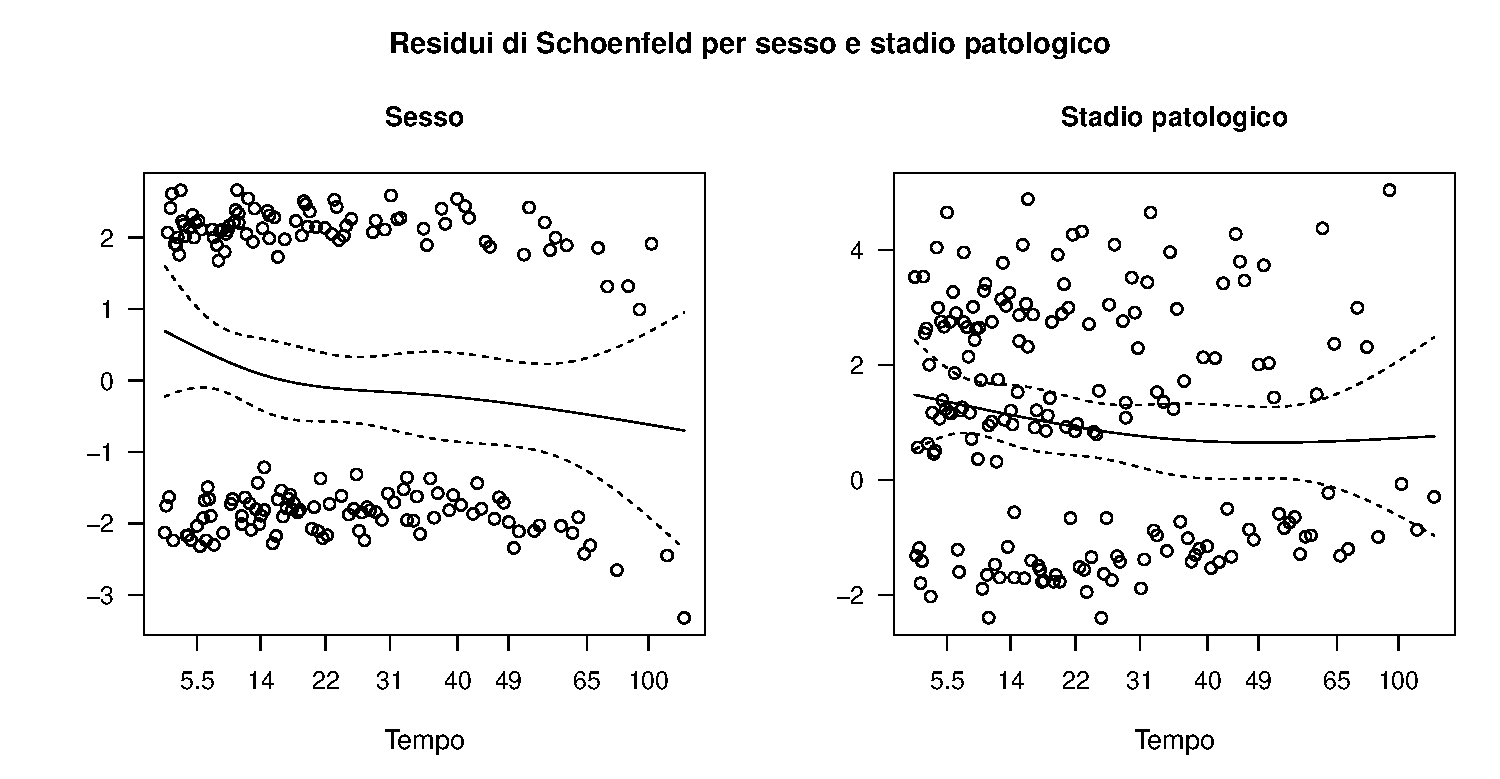
\includegraphics[width=0.95\textwidth]{schoenfeld_sesso_stadio.pdf}
\caption{Residui di Schoenfeld per sesso e stadio patologico.}
\label{fig:schoenfeld_sesso_stadio}
\end{figure}

I grafici confermano che l'effetto del sesso e dello stadio patologico non rimane costante durante il follow-up. In particolare, le curve smussate dei coefficienti stimati mostrano un andamento non perfettamente orizzontale nel tempo, coerente con i risultati significativi del test di Schoenfeld.

Poiché l'ipotesi di rischi proporzionali non risulta soddisfatta per queste due covariate, è stato successivamente stimato un modello di Cox stratificato per sesso e stadio patologico. In questo modo, ciascuna combinazione delle due variabili può avere una propria funzione di rischio di base, senza imporre un effetto costante nel tempo.

\subsubsection{Modello di Cox stratificato}

Per gestire la violazione dell'ipotesi di proporzionalità è stato stimato un modello di Cox stratificato congiuntamente per stadio patologico e sesso. La stratificazione consente a ciascuna combinazione di stadio e sesso di possedere una propria funzione di rischio di base, senza imporre che gli effetti di queste due variabili rimangano costanti durante il follow-up.

Il modello finale è:

\begin{equation}
h_s(t \mid X)
=
h_{0s}(t)
\exp\{
\beta_1 \mathrm{Et\grave{a}}_{10}
+\beta_2 \mathrm{Istologia}
+\beta_3 \mathrm{Buffa}_{10}
\},
\label{eq:cox_stratificato}
\end{equation}

dove $s$ identifica lo strato definito dalla combinazione tra stadio patologico e sesso. La stratificazione consente quindi funzioni di rischio di base differenti per le combinazioni osservate delle due variabili, fino a un massimo teorico di otto strati. Il costo di questa scelta è che il modello non restituisce un unico hazard ratio per sesso e stadio patologico, poiché i loro effetti vengono assorbiti nelle funzioni di rischio di base specifiche di strato.

I risultati del modello stratificato finale sono riportati nella Tabella~\ref{tab:cox_stratificato}.

\begin{table}[H]
\centering
\caption{Modello di Cox stratificato per stadio patologico e sesso.}
\label{tab:cox_stratificato}
\renewcommand{\arraystretch}{1.15}
\small
\begin{tabular}{l c c c}
\toprule
\textbf{Covariata}
& \textbf{HR}
& \textbf{IC 95\%}
& \textbf{$p$-value} \\
\midrule
Età, per 10 anni
& 1,241
& 1,055--1,460
& 0,009 \\

Adenocarcinoma misto vs NOS
& 0,769
& 0,516--1,144
& 0,195 \\

Altri sottotipi vs NOS
& 0,473
& 0,275--0,812
& 0,007 \\

Buffa score, per 10 punti
& 1,107
& 1,025--1,196
& 0,010 \\
\bottomrule
\end{tabular}
\end{table}

Il modello stratificato risulta globalmente significativo secondo il likelihood ratio test ($p<0,001$).

Anche dopo aver consentito a stadio e sesso di possedere rischi di base differenti, l'età e il Buffa Hypoxia Score rimangono significativamente associati alla sopravvivenza. Un aumento di dieci anni nell'età determina un incremento dell'hazard pari a circa il 24,1\%, mentre un aumento di dieci punti del Buffa score è associato a un incremento del rischio pari al 10,7\%.

Gli altri sottotipi istologici continuano a mostrare un hazard inferiore rispetto all'adenocarcinoma NOS, mentre l'adenocarcinoma misto non presenta una differenza statisticamente significativa.

\subsubsection{Verifica del modello stratificato}

Il test di Schoenfeld è stato ripetuto sulle covariate stimate nel modello stratificato. I risultati sono riportati nella Tabella~\ref{tab:schoenfeld_stratificato}.

\begin{table}[H]
\centering
\caption{Test di Schoenfeld per il modello di Cox stratificato.}
\label{tab:schoenfeld_stratificato}
\renewcommand{\arraystretch}{1.15}
\begin{tabular}{l c c c}
\toprule
\textbf{Covariata}
& \textbf{Chi-quadro}
& \textbf{gdl}
& \textbf{$p$-value} \\
\midrule
Età
& 2,796
& 1
& 0,095 \\

Sottotipo istologico
& 0,167
& 2
& 0,920 \\

Buffa Hypoxia Score
& 0,191
& 1
& 0,662 \\

\textbf{Globale}
& \textbf{3,613}
& \textbf{4}
& \textbf{0,461} \\
\bottomrule
\end{tabular}
\end{table}

Tutti i valori di $p$ risultano superiori a 0,05 e il test globale non è significativo. Non emerge quindi evidenza di una violazione residua dell'ipotesi di rischi proporzionali. Per questo motivo non vengono riportati ulteriori grafici dei residui di Schoenfeld per il modello stratificato.

Il modello stratificato viene pertanto considerato il modello finale, poiché consente di gestire la non proporzionalità di sesso e stadio mantenendo nel modello le associazioni relative all'età, al sottotipo istologico e all'ipossia tumorale. Tale scelta comporta tuttavia la rinuncia alla stima di un unico hazard ratio per le due variabili utilizzate nella stratificazione.

\subsection{Diagnostica del modello definitivo}

Per valutare l'adeguatezza della forma funzionale delle covariate continue incluse nel modello stratificato finale sono stati analizzati i residui di Martingala rispetto all'età e al Buffa Hypoxia Score.

\begin{figure}[H]
\centering
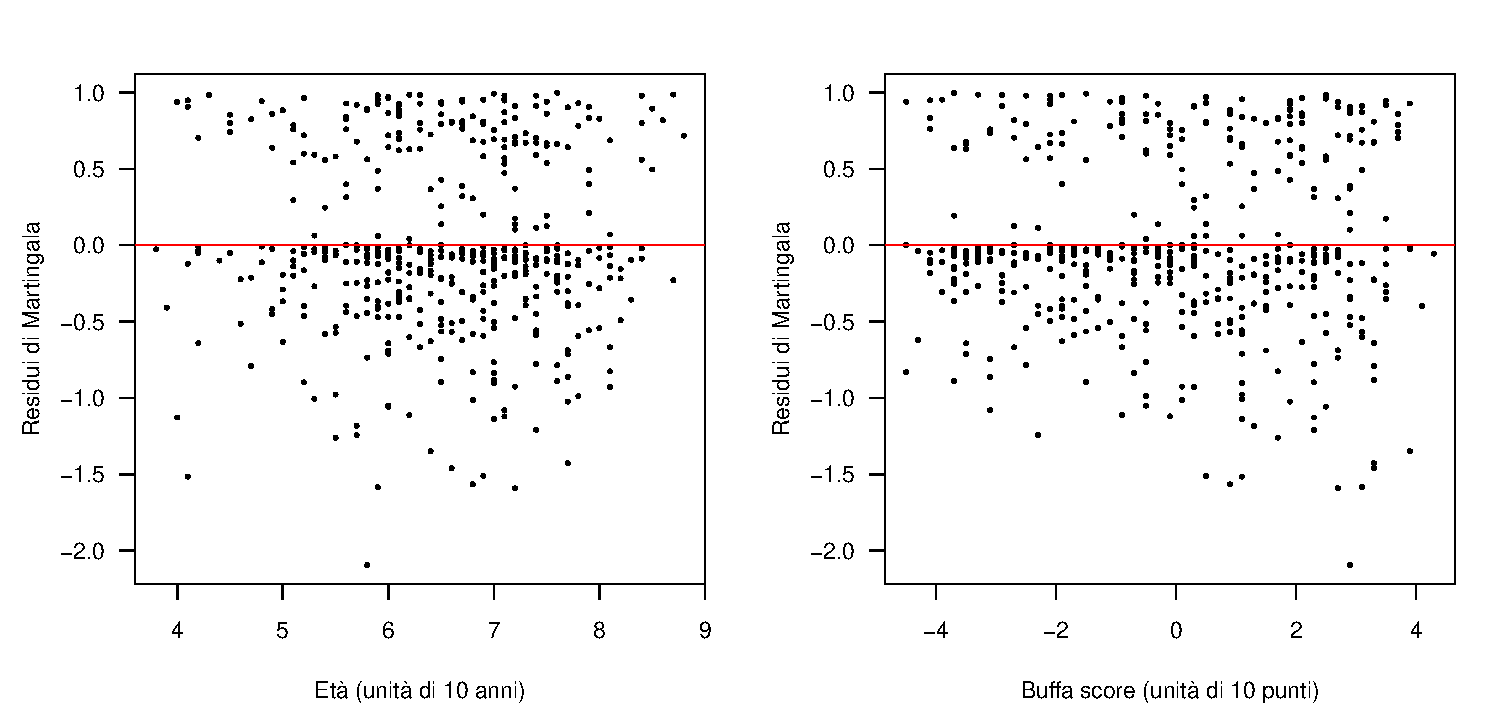
\includegraphics[width=0.95\textwidth]{martingala_eta_buffa.pdf}
\caption{Residui di Martingala rispetto all'età e al Buffa Hypoxia Score.}
\label{fig:martingala_eta_buffa}
\end{figure}

La linea rossa orizzontale rappresenta il valore di riferimento pari a zero. In entrambi i grafici i residui risultano dispersi al di sopra e al di sotto di tale linea, senza evidenziare pattern sistematici particolarmente marcati rispetto all'età o al Buffa Hypoxia Score. L'analisi grafica non suggerisce quindi deviazioni evidenti dalla forma funzionale lineare adottata nel modello.

\subsection{Profili prognostici clinico-molecolari}

Per illustrare l'effetto congiunto dell'età e dell'ipossia tumorale sono stati definiti tre profili ipotetici. Il profilo favorevole corrisponde a una paziente di 55 anni con Buffa Hypoxia Score pari a $-20$, quello intermedio a una paziente di 65 anni con score pari a 0 e quello sfavorevole a una paziente di 75 anni con score pari a 20. In tutti e tre i profili sono stati mantenuti costanti il sesso femminile, lo stadio I e il sottotipo istologico Adenocarcinoma NOS.

\begin{figure}[H]
\centering
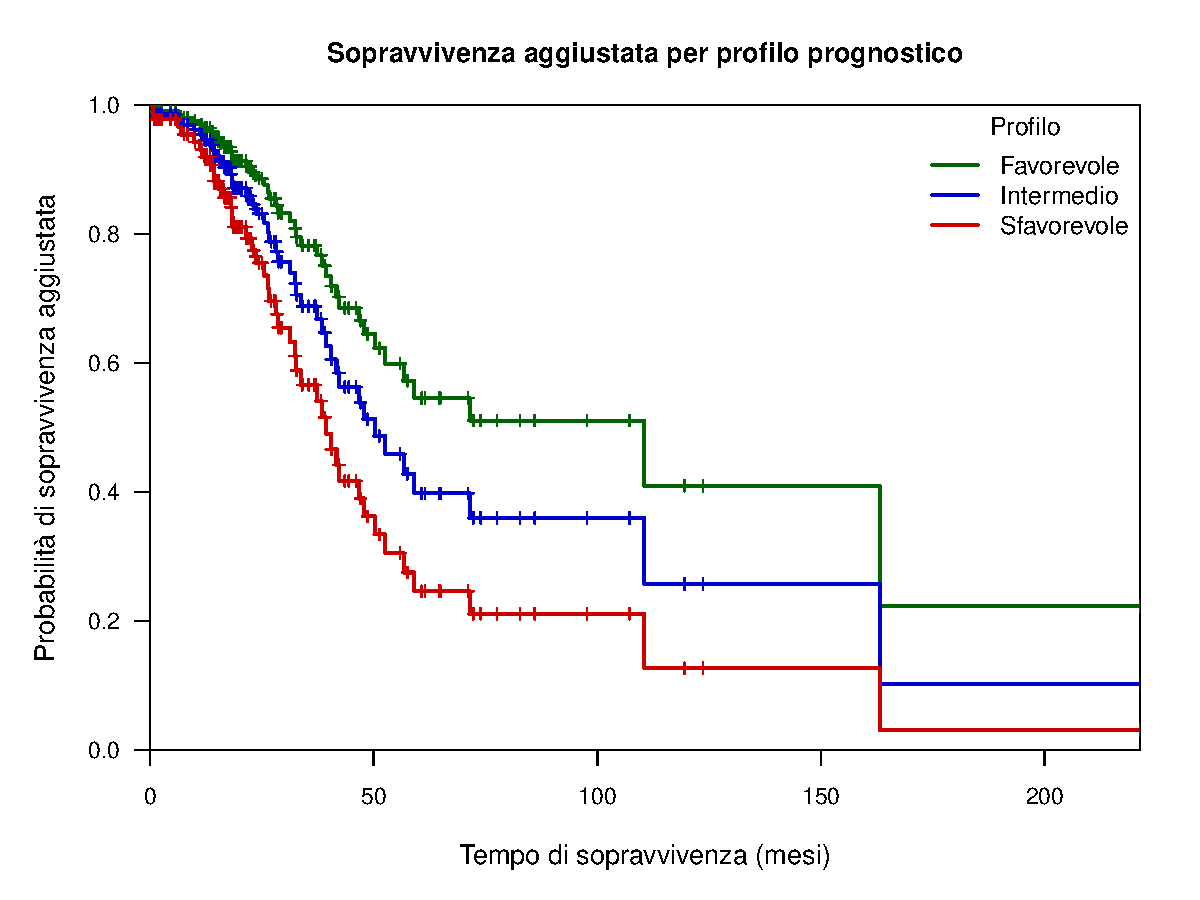
\includegraphics[width=0.95\textwidth]{curve_profili_prognostici.pdf}
\caption{Curve di sopravvivenza stimata per i tre profili prognostici clinico-molecolari.}
\label{fig:profili_prognostici}
\end{figure}

Le curve mostrano un gradiente prognostico netto. A 60 mesi, la sopravvivenza stimata è pari a 0,546 per il profilo favorevole, 0,398 per quello intermedio e 0,246 per quello sfavorevole. La separazione riflette l'effetto combinato di età e Buffa Hypoxia Score secondo il modello stimato.

\section{Limiti dello studio}

I risultati devono essere interpretati considerando alcuni limiti. In primo luogo, l'analisi utilizza dati osservazionali e retrospettivi, per cui le associazioni stimate non possono essere interpretate in senso causale. Inoltre, è stata adottata un'analisi per casi completi: la quota di osservazioni escluse è contenuta, ma la validità delle stime richiede che i dati mancanti non introducano differenze sistematiche rilevanti tra pazienti inclusi ed esclusi.

La numerosità dello stadio IV è ridotta e la stratificazione congiunta per stadio e sesso suddivide ulteriormente il campione in combinazioni meno numerose. Le stime relative agli strati meno rappresentati devono quindi essere interpretate con cautela. Infine, la categoria ``Altri sottotipi'' riunisce forme istologiche differenti e può nascondere una certa eterogeneità interna.

\section{Conclusioni}

L'analisi evidenzia che età alla diagnosi, Buffa Hypoxia Score e sottotipo istologico sono associati alla sopravvivenza dei pazienti con adenocarcinoma polmonare. In particolare, un aumento di dieci anni nell'età corrisponde a un incremento dell'hazard di circa il 24\%, mentre un aumento di dieci punti del Buffa score è associato a un incremento di circa l'11\%.

Lo stadio patologico risulta fortemente associato alla prognosi nel modello standard. Poiché sesso e stadio non soddisfano l'ipotesi di rischi proporzionali, è stato adottato un modello stratificato, che elimina l'evidenza di violazioni residue e mantiene le associazioni relative alle altre covariate.

Nel complesso, i risultati indicano che l'integrazione tra caratteristiche cliniche e ipossia tumorale consente di distinguere livelli prognostici differenti, pur con i limiti legati alla natura osservazionale dei dati e alla ridotta numerosità di alcuni sottogruppi.

\section{Fonti}

I dati utilizzati nell'analisi provengono dallo studio
\textit{Lung Adenocarcinoma (TCGA, PanCancer Atlas)}, disponibile su cBioPortal for Cancer Genomics:

\begin{center}
\href{https://www.cbioportal.org/study/summary?id=luad_tcga_pan_can_atlas_2018}
{\texttt{https://www.cbioportal.org/study/summary?id=luad\_tcga\_pan\_can\_atlas\_2018}}
\end{center}

\end{document}